\documentclass{../src/bcthesispart}
\title{A discrete Weibull model of population turnover}
\author{Bas Cornelissen}
\begin{document}

%——————————————————————————————————————————————————————————

\appendixtitle{A discrete Weibull model of population turnover}%
	{A discrete Weibull model of population turnover}%
	{weibull}{%
	%
	% Abstract
	% ————————
	Population turnover is commonly modelled by replacing one random agent in every round. 
	Such a constant mortality rate is not very realistic, and this appendix proposes an alternative, discrete Weibull model.
	It is reparametrised such that the mean life expectancy is the only parameter.
}

%——————————————————————————————————————————————————————————




\noindent
How can we realistically model the mortality-rate in a population?
This is a central question in \emph{survival analysis} \parencite[e.g.][]{Rodriguez2007}.
In the context of a model of language evolution, if one agent dies in every iteration, the probability that any given agent dies at time $t$ is thus $\gamma$ — \emph{given that it was still alive at time $t-1$}.
If $T$ is the random variable that measures the time of death of an agent, this means $p(T = t \mid T \ge t) = \gamma$.
This conditional probability is known as the \emph{hazard rate} $h(t)$, as it measures the rate of death (hazard) occurring at $t$.\footnote{%
	%>>>
	It is usually defined for continuous $T$ with density $f$ as $h(t) = \frac{f(t)}{1-F(t)}$, in which case it is not a conditional probability but the \emph{rate} of instantaneous hazard.
	%<<< 
	}
In our example the hazard rate was constant.
But, as explained in chapter \ref{ch:bayesian-naming-games}, models with constant hazard rates are poor models of life-expectancy in human populations and demographers usually adopt either the \emph{Weibull} or \emph{Gompertz} distribution \parencite{Juckett1993}.
We here consider the simpler Weibull distribution, mainly because several discrete analogous have been proposed \parencite{Nakagawa1975,Stein1984,Almalki2014}.




%——————————————————————————————————————————————————————————
\paragraph{Discrete Weibull distribution} 

The Weibull distribution \parencite{Weibull1951} is a continuous distribution parametrized by a scale parameter $\kappa>0$ and a shape parameter $\lambda>0$. 
If $\kappa>1$ the distribution is unimodal, meaning that most agents die around the same age, which is in turn determined by $\lambda$ (see figure \ref{fig:weibull-params}).
For completeness, the density of a Weibull-distributed random variable $T$ is
\begin{align}
	p(t \mid \lambda, \kappa) = \nicefrac{\kappa}{\lambda} \cdot \bigr(\nicefrac{t}{\lambda}\bigl)^{\kappa-1} \cdot \;\text{exp}\Bigl(-\bigr(\nicefrac{t}{\lambda}\bigl)^{\kappa}\Bigr).
\end{align}
Since language games are discrete time models, we use a discrete approximation known as the \emph{Discrete Weibull} distribution\footnote{I reparametrized the distribution by taking $\beta := \kappa$ and $q := \text{exp} ( - \lambda^{-\kappa})$, which is both computationally and conceptually more convenient.}\parencite{Nakagawa1975}, which preserves the so called \emph{survival} function of the continuous distribution.
The \emph{survivor} function $S(t) = p(T \ge t)$ measures the probability of surviving to at least time $t$.
The Weibull distribution, this function takes the form
\begin{equation}
	S(t) = \text{exp}\Bigl(	-\bigl(\nicefrac{t}{\lambda}\bigr)^k\Bigr),
\end{equation}
and the Discrete Weibull is defined as the discrete distribution with the same survival function.
This can be done, since the probability mass function is fully determined by the survival function:
\begin{equation}
p(T = t) = S(t) - S(t+1) = \text{exp}\Bigl(	- \bigl(\nicefrac{t}{\lambda}\bigr)^\kappa \Bigr) - \text{exp}\Bigl(- \bigl(\nicefrac{t+1}{\lambda}\bigr)^\kappa\Bigr).
\end{equation}
It should be stressed that the resulting distribution \emph{approximates} the Weibull distribution, which for our purposes is sufficient.




The hazard rate of the Discrete Weibull distribution can be computed as
\begin{align}
	h(t) 
		= p(T= t \mid T\ge t)
		= \frac{S(t) - S(t+1)}{S(t)}
		= 1 - \text{exp}\Bigl( \bigl(\nicefrac{t}{\lambda}\bigr)^{\kappa} -  \bigl(\nicefrac{t+1}{\lambda}\bigr)^{\kappa}\Bigr).
\end{align}
Recall that the hazard rate is the probability that an agent dies at time $t$, given that it hasn’t died yet. 
Therefore, if we want to model a population where the probability of dying at time $T$ approximately follows a Weibull distribution, we should in every round flip a coin with weight $h(t)$ to decide whether the agent dies. 




%- - - - - - - -
\begin{SCfigure}
	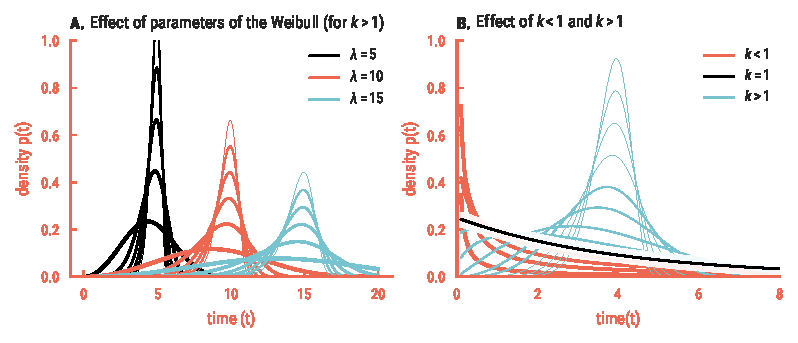
\includegraphics[trim=1.2cm 0 0 \figtopmargin]{FIG04-Weibull-params}
	\caption{
	The Weibull distribution can model the probability that an agent dies at time $t$.
	\subfig{A} Varying the parameters of a Weibull distribution illustrates that $\lambda$ is a scale parameter and $\kappa$ a shape paramater.
	\subfig{B} If $\kappa>1$ the Weibull is a unimodal distribution, whose variance decreases with higher $\kappa$ (thinner lines), but for $\kappa<1$ the distribution has no mode.
	When $\kappa=1$ the Weibull reduces to a exponential distribution.
		\figdetails{\figid{fig04}}
		\label{fig:weibull-params}}
\end{SCfigure}
%- - - - - - - -

%- - - - - - - -
\begin{SCfigure}
	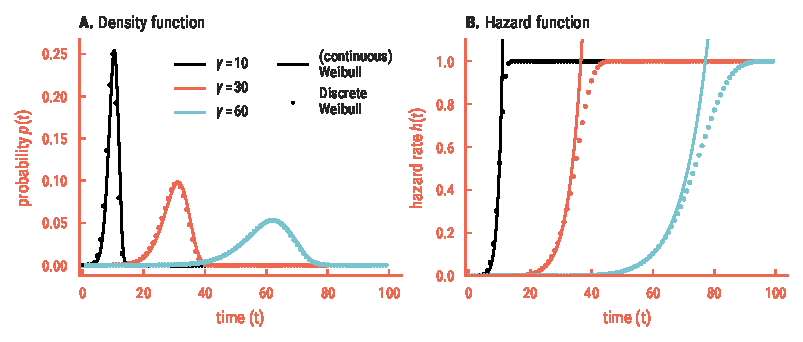
\includegraphics[trim=1.33cm 0 0 \figtopmargin]{FIG04-continuous-discrete-Weibull}
	\caption{The single-parameter version of the continuous and discrete Weibull distribution. 
		\subfig{A} The distributions closely line up and $\gamma$ is easily interpretable. 
		\subfig{B} The hazard rate increases with time, thus capturing ageing effects. 
		Note that a continuous hazard rate $h(t)$ is not a distribution and exceeds 1.
		\figdetails{\figid{fig04}}
		\label{fig:cont-discr-weibull}}
\end{SCfigure}
%- - - - - - - -




%——————————————————————————————————————————————————————————
\paragraph{Modelling population turnover}

The Discrete Weibull gives us a more realistic model of population turnover, but its behaviour is regulated by two parameters: $\lambda$ and $\kappa$.
Ideally a \emph{single} parameter would interpolate between immediate death (iterated learning) and immortality (naming game).
This can be done by defining $\lambda$ and $\kappa$ in terms of a $\gamma \ge 1$:
\begin{align}
	\kappa(\gamma) := \log(\gamma) + \kappa_0
	\qquad\text{and}\qquad
	\lambda(\gamma) := \frac{\gamma}{\Gamma\bigl(1 + \nicefrac{1}{\kappa(\gamma)}\bigl)}, \qquad \gamma\ge1
\end{align}
where $\Gamma$ is the gamma function. 
Figure \ref{fig:cont-discr-weibull} illustrates the effect of $\gamma$.
Three reasons underly this reparametrization. 
First, the term $\Gamma\bigl( 1 + \nicefrac{1}{\kappa(\gamma)}\bigl)$ makes $\gamma$ interpretable: $\gamma$ is the mean of the continuous distribution $\text{Weibull}\bigl(\lambda(\gamma), \kappa(\gamma)\bigl)$.
Second, scaling $\kappa(\gamma)$ logarithmically with $\gamma$ results in a realistic mortality distribution for all $\gamma\ge 1$.
Third, the constant $\kappa_0$ guarantees that for $\gamma=1$ the hazard rate is approximately 1, corresponding to instant death in iterated learning. I opt for\footnote{This results in the hazard rate $h(1 \mid \lambda=1) > 1 - 10^{-8}$, which seems sufficiently close to 1.} $\kappa_0 = 5$.




In sum, we have defined a discrete Weibull model, approximating the continuous Weibull, but parametrised by a single parameter $\gamma$, the average life expectancy. 
When used in combination with a random walk through a population of fixed size, $\gamma$ thus interpolates between iterated learning ($\gamma=1$) and a naming game ($\gamma=\infty$).




%——————————————————————————————————————————————————————————
\showbibliography

\end{document}
